\chapter{Background and theoretical framework}
\section{Valency and valency phenomena}

% valency - terminology introduction

In chemistry, \textit{valency}, or \textit{valence}, refers to the combining power of an atom or radical. The valency of any atom can be measured by the number of hydrogen atoms that it can combine with or displace in a chemical compound \citep{law2020a}. This same term was introduced to linguistics by analogy and refers to the combining power of a word, primarily a verb or predicate, with other words or elements of the sentence. 

Lucien Tesnière is generally credited with introducing the term valency to linguistics with his syntactic theory of valency and dependence, as presented in the posthumously published \textit{Éléments de syntaxe structurale} (\cite*{tesniere1959}; English translation \cite*{tesniere2015}).\footnote{
    It should be noted that while Tesnière is rightly credited with the introduction of a theory of linguistic valency, the metaphor of valency itself has made appearances as early as in \citet{peirce1897}, among others \citep{przepiorkowski2018}.
}
In another of Tesnière's analogies, each verbal node, being the center of sentence structure, is not unlike a ``theatrical performance'' with the verb expressing the process and the nouns being the \textit{actants} (what we would now call \textit{arguments}) in this performance. Just like how atoms of different elements allow for a greater or lesser number of bonds, different verbs can combine with a greater or lesser number of actants, i.e., their valency.

% the phenomena now we are now calling valency - different theories
While the term valency is borrowed into linguistics from chemistry, the study of the phenomena which are covered by or otherwise overlap with valency has a much longer tradition, dating to the early beginnings of linguistics from the kāraka concept of semantic relation between verb and noun \citep{ganeri2011a} in Pāṇinian grammar to modern case grammar \citep{fillmore1968}. 

Implicit in the focus on verbal valency is the assumption, shared by most linguistic theories, of the centrality of the verb in determining either or both the syntactic and semantic structure of a sentence. This assumption has also been corroborated by psycholinguistic evidence \citep{healy1970} and places valency and the issues of \textit{argument structure} squarely at the center of the inquiry into the interface between syntax and lexical semantics.

%% subcategorization in generative grammar
In generative grammar, the syntactic valency of a verb is treated under a similar notion of \textit{subcategorization} \citep{chomsky1965a}. As an example, a transitive verb must be followed by a direct object, whereas an intransitive verb cannot. As such, transitive and intransitive verbs form subcategories of the category of verb. Verbs are thus further assigned to \textit{subcategorization frames} which specify the number and type of complements, i.e., objects and obliques, (and of subjects as well in later theories), that the verb can be subcategorized for. In addition to being syntactically driven, a notable feature of generative theories' treatment of valency is that the subcategorization frames are considered as part of the lexical entry of the verb. Later work in generative grammar, in particular \citet{jackendoff1972,jackendoff1987,jackendoff1992}, following \citet{katz1963} and \citet{gruber1962}, further developed a theory of thematic relations and posited that argument structure serves as the interface between syntactic and thematic structures.
% unclear on relationship between subcategorization and selection in generative grammar; also maybe more citations and examples here later

%% Levin
As compared to broader distinctions such as those made between transitive and intransitive verbs, \citet{levin1993} categorized verbs in a much more fine-grained manner based on their syntactic behavior into different verb classes. Starting from the assumption that the syntactic behavior of verbs are determined semantically, Levin reasons that patterning together classes of verbs based on their diathesis alternations should result in semantically coherent verb classes. Levin's work has been highly influential both in the development of valency theory, where it spurred further work on verb classes, and in computational approaches to lexical semantics, where the VerbNet \citep{kipper-schuler2005, kipper2006, kipper2008} is a prominent example of projects extending the Levin verb classes into a computational lexicon that links with other resources such as WordNet \citep{fellbaum1998, miller1995}, PropBank \citep{kingsbury2002}. Further work on verb class induction based on syntactic patterns includes \citet{basili1993, navarretta2000, korhonen2006, sun2008, sun2009,sun2013} in English, \citet{schulteimwalde2002, schulteimwalde2003, schulteimwalde2006} in German, \citet{snider2006} in Arabic. \citet{sun2013} in particular included diathesis alternation as input feature. Other work focused instead on the induction of semantic verb classes such as \citet{furstenau2012, majewska2018, majewska2020}. And work such as \citet{dowty1991, abend2009, titov2012, bickel2014, sayeed2018, watanabe2010, yamada2021}, among others, worked on the induction of semantic roles, a topic arguably tightly related to the induction of the verb classes.
 
%% frame semantics - fillmore
Another computational project focused on verbal valency, FrameNet \citep{baker1998, fillmore2015} differs from VerbNet in terms of their theoretical foundations, in that it derives from a divergent line of research that stemmed from Charles Fillmore's frame semantics \citep{fillmore1977, fillmore1977a, fillmore1982}, which in turn has its roots in his earlier work on case grammar \citep{fillmore1968,fillmore1970}. While they are often computationally interoperable to some extent, there remains a key conceptual distinction made in frame semantics \citet{fillmore1968}, namely the \textit{frames}-driven analysis of argument encoding. While the verbal lexicon continues to play a role in placing selectional restrictions on the frames in which a given verb can be found in, the frames are themselves said to have semantics through their grouping of frame elements, which are similar to thematic roles but local to their specific frames. The frame semantics approach is consolidated by further development in construction grammar where the frames are viewed as a level of constructions on their own, cf. e.g., \citet{goldberg1992,goldberg1995}'s \textit{argument structure constructions}. Furthermore, construction grammar theories often argue for frames to be considered distinct or autonomous constructions, as it is not strictly predictable from other constructions.

\section{Typological perspectives on valency and dependency}

It is perhaps not surprising that, besides introducing the analogy of valency, \citet{tesniere1959} also introduced the notion of dependency into modern linguistics. In terms of their mathematical foundations, dependency grammar, based on the notion of dependencies, can be viewed in contrast with constituency grammars which are based on the notion of substitution instead \citep{stabler2019}. However, even most iterations of generative grammar theories, which are primarily constituency-based, incorporate some version of a head-dependent relationship (cf. X-bar theory). \citet{demarneffe2019} cited the easiness of generalization across languages, its operationalization of human sentence processing facts, and the transparency and simplicity of representation as reasons why dependency-based representations have become increasingly widely adopted in linguistic theory and even more so in NLP.

The usefulness of dependency grammar in allowing for cross-lingual generalizations and comparisons of linguistic structures should not be understated. Universal Dependencies (UD) \citep{nivre2015,demarneffe2021} in particular is an initiative that aims to develop a uniform grammatical annotation system that are cross-lingually consistent. The basic structure of the UD annotation is to segment \textit{sentences} into \textit{syntactic words} which are annotated with their \textit{morphological properties} and linked together by \textit{syntactic relations}. A comparison of UD annotations of equivalent sentences in two languages shows how they can show both the structural parallel and differences between how two languages encode the same sentence, as seen in Fig.~\ref{fig:ud-example-sentence}, where both the similarities between how English and Finnish encoded semantically equivalent sentences (same syntactic relationships between the arguments and the verb) and the differences (case markings in Finnish, preposition in English) are easily discernable. And further enhancements have also been proposed that would make the UD annotation scheme more compatible with contemporary typological theory \citep{croft2017}.

\begin{figure}
    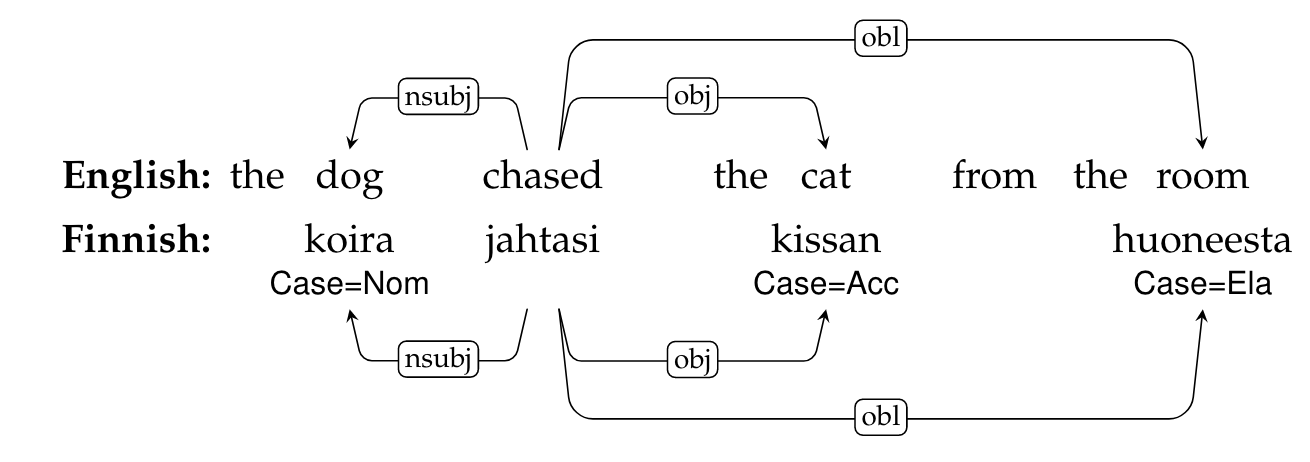
\includegraphics[width=0.85\textwidth]{figures/ud_example_sentence.png}
    \centering
    \caption{Simplified UD annotation for equivalent sentences from English (top) and Finnish (bottom) \citep{demarneffe2021}.}\label{fig:ud-example-sentence}
\end{figure}

Specifically on verbal valency, already \citet{tesniere1959} was paying attention to the cross-lingual differences in the argument structure of semantically equivalent sentences while describing his dependency grammar. Tesnière described the process of \textit{metataxis}, by which syntactic structures of one language are ``translated'' to those of another. Such a process points to the clear typological interest in valency systems, namely the mismatch between how languages encode their argument structure.

\todo{transitivity}

% focus on markedness hierarchy
In terms of possible universals that can be observed, \citet{tsunoda1981, tsunoda1985} proposed a transitivity hierarchy of verbs:
\begin{quote}
    Effective action >> Perception >> Pursuit >> Knowledge >> Feeling >> Relation
\end{quote}
The idea is that languages that encode verbs that are lower in this hierarchy as transitive verbs will encode all those above them too as transitive, with the effective action being the most prototypical transitive verb, hence most likely to be transitive in a language. This approach is further extended by \citet{malchukov2005} who used the semantic map method and proposed a two-dimensional transitivity hierarchy with the semantic map method. 

There has been some recent work from advocates of both the lexeme- and frames-based approaches on the cross-lingual alignment of their respective units of linguistic analysis. On the frames-based side, \citet{baker2020, ellsworth2021} explored the cross-lingual alignment of frames based on FrameNet; in contrast, \citet{say2014} rejected the equating of minor valency classes cross-lingually and studied how verb classes compare cross-lingually instead, seeing that as a more valid method of measuring how languages organize their verbal lexicon differently.
